\def\conf{0}
% * <themis.gouleakis@gmail.com> 2015-10-09T19:27:57.769Z:
%
% 
%
\def\icalp{0}
\def\both{0}

\documentclass[11pt]{article}
\usepackage{fullpage}


\usepackage{graphicx,amsfonts,amsmath,amssymb,epsfig,hyperref,color}
\usepackage{algorithm}
\usepackage{pdfpages}
\usepackage{enumitem}
\usepackage{multirow}
\usepackage{thm-restate}

\usepackage{mathtools}

\usepackage[noend]{algpseudocode}
\usepackage[english]{babel}
\usepackage[utf8]{inputenc}
\usepackage{amsmath}
\usepackage{graphicx}
\usepackage[colorinlistoftodos]{todonotes}

\usepackage{verbatim}
\usepackage{comment}
\usepackage{hyperref}

\usepackage{boxedminipage}
\usepackage{fullpage}
\usepackage{array}
\usepackage[normalem]{ulem}

\usepackage{relsize}
\usepackage{amsthm}

%\usepackage{amsmath,amssymb,amsthm}
%\theoremstyle{definition}
%\newtheorem{defn}{Definition}
%\newtheorem{ques}{Question}

%\theoremstyle{remark}
%\newtheorem{obs}{Observation}
%\newtheorem{rem}{Remark}

%\theoremstyle{definition}
\newtheorem{lemma}{Lemma}
\newtheorem{claim}{Claim}
\newtheorem{theorem}{Theorem}
\newtheorem{definition}{Definition}
\newtheorem{corollary}{Corollary}
\newtheorem{proposition}{Proposition}

\setlength{\parindent}{0pt}
\setlength{\parskip}{1em}

\def\ll{\left}
\def\rr{\right}
\def\RR{\mathbb{R}}
\def\ee{\mathbb{E}}
\def\pp{\mathbb{P}}
\def\bo{\mathcal{O}}
\def\Bo{\mathlarger{\mathcal{O}}}
\def\bt{\Theta}
\def\polylog{\mathrm{polylog}\;}

\DeclarePairedDelimiter\floor{\lfloor}{\rfloor}
\newcommand{\SL}[2]{\sum\limits_{#1}^{#2}}
\newcommand{\BSL}[2]{\mathlarger{\mathlarger{\sum}\limits_{#1}^{#2}}}
\newcommand{\PL}[2]{\prod\limits_{#1}^{#2}}
\newcommand{\BPL}[2]{\mathlarger{\mathlarger{\prod}\limits_{#1}^{#2}}}

\newcommand{\anak}[1]{\todo[inline,color=green]{Anak: #1}}

%\usepackage{hyperref}
\usepackage{multirow}

\usepackage[margin=10pt]{subfig}

\usepackage{graphicx}
\usepackage{colortbl}
\newcommand{\lemautorefname}{Lemma}
\usetikzlibrary{
  shapes.multipart,
  matrix,
  positioning,
  shapes.callouts,
  shapes.arrows,
  calc}


\title{Distributed Density Estimation} 

\date{}
%\author{
%Amartya Shankha Biswas
%\thanks{MIT, Cambridge MA 02139.
%E-mail: {\tt  asbiswas@mit.edu}.}
%}


\begin{document}


\maketitle

%\section{Miscellaneous Results}
%\label{sec:miscellaneous_results}

%\subsection{Domino Tiling}
We will consider the problem of tiling a square grid with dominos.
This problem has a long histor and various importtant applications in statistical physics.
Specifically, we will focus on the local generation of domino tilings from the uniform distribution.

\subsection{$2\times n$ Domino Tiling}
The simplest version of the problem is one where we are given a $2\times n$ grid (Figure~\ref{fig:dom2}.
The queries will be as an index, and the generator should report the orientation of the domino at the $i^{th}$ position in the grid.
\begin{figure}[htbp]
    \centering
    %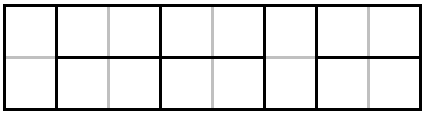
\includegraphics[width=\textwidth]{images/domino2}
    \caption{}
    \label{fig:dom2}
\end{figure}

It is a well known result \todo{cite} that the number of tilings of a $2\times n$ grid is exactly $F_n$.

To aid with generalization, we will instead allow the generator to respond with the splitting boundary of the current tiling instead.
For example, in Figure~\ref{fig:b20}, the boundary is a vertical line at the specified position.
In Figure~\ref{fig:b21}, the boundary is horizontal, indicating that there are two horizontal dominos at that location.
Note that Figure~\ref{fig:b22} is impossible for a $2\times n$ grid.
It should be clear that this query model is equivalent.

\begin{figure}[h]
    \centering
    \subfloat[][]{
        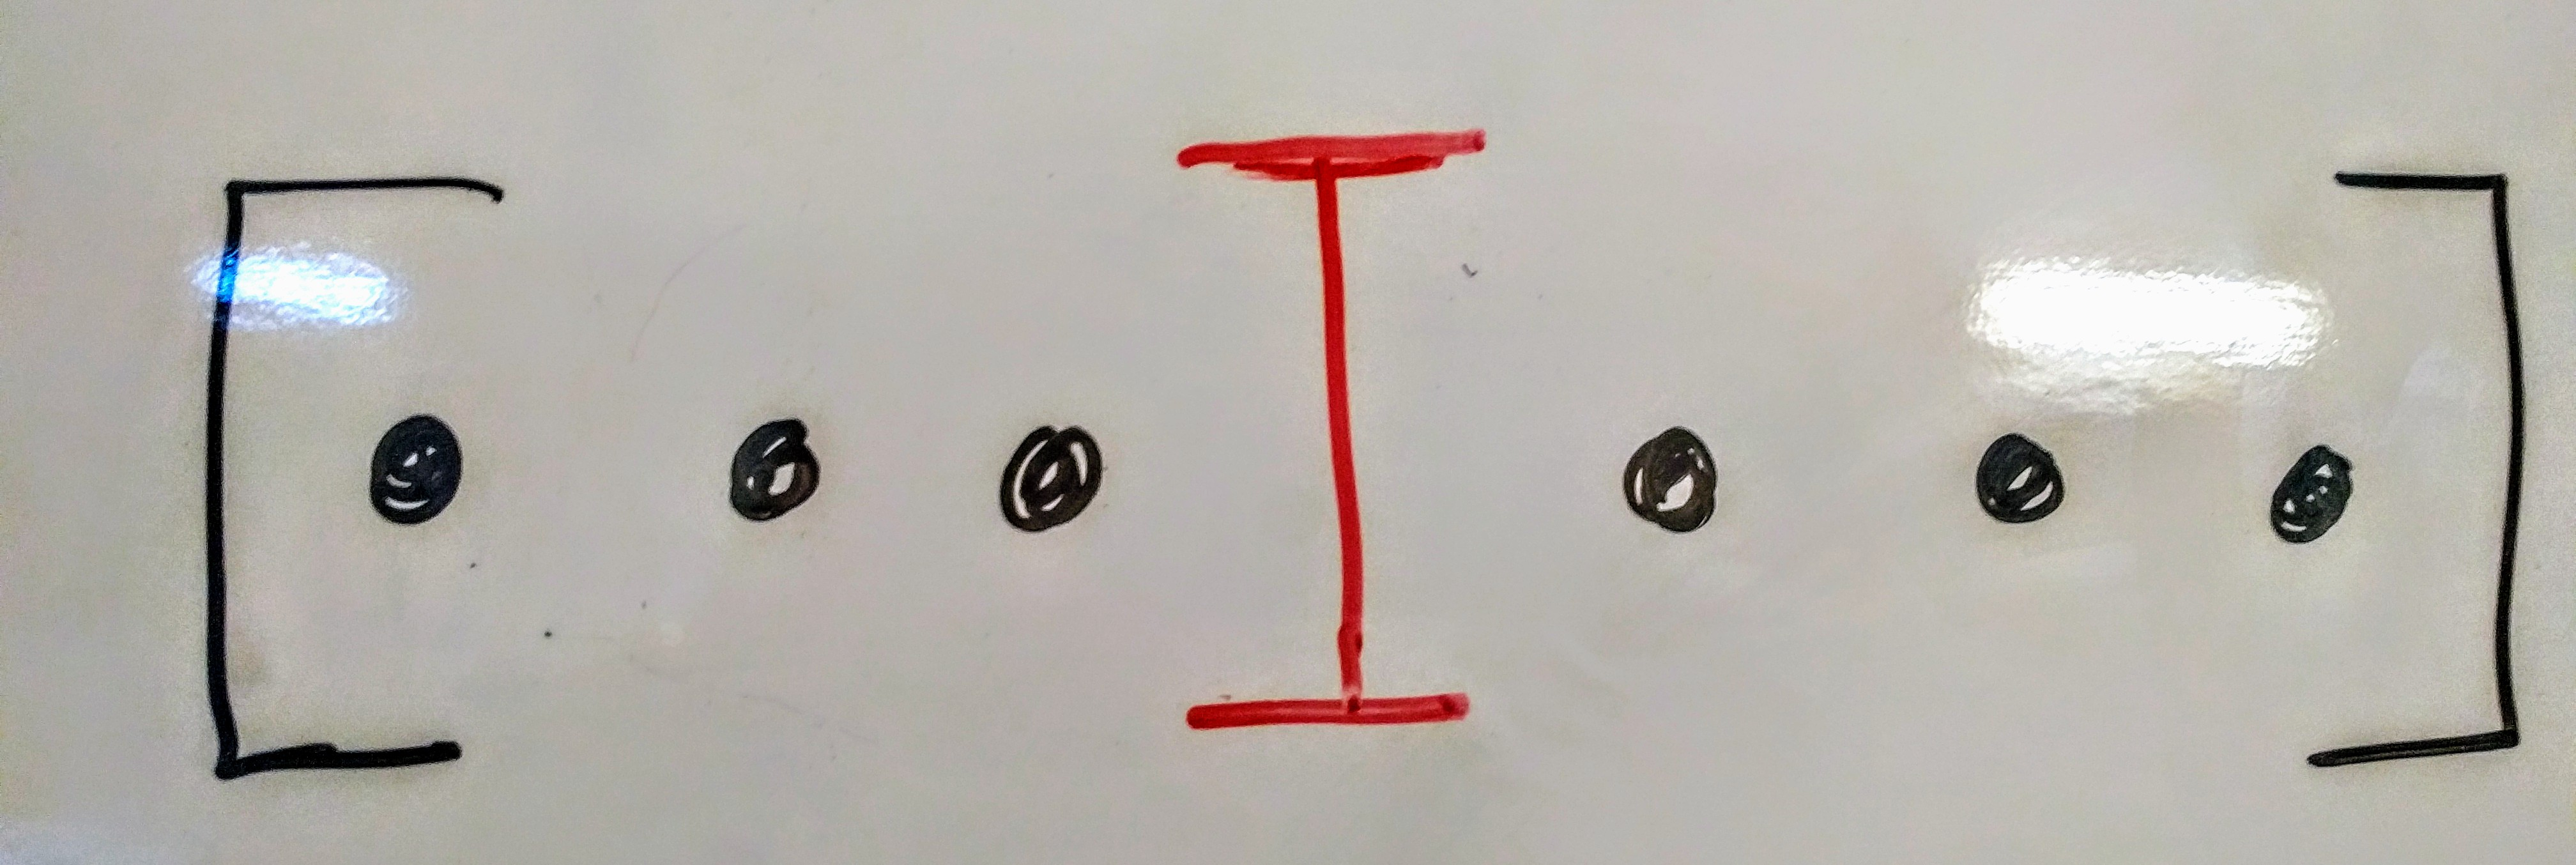
\includegraphics[width=0.5\linewidth]{images/tile2-0.jpg}
        \label{fig:b20}
    }
    \subfloat[][]{
        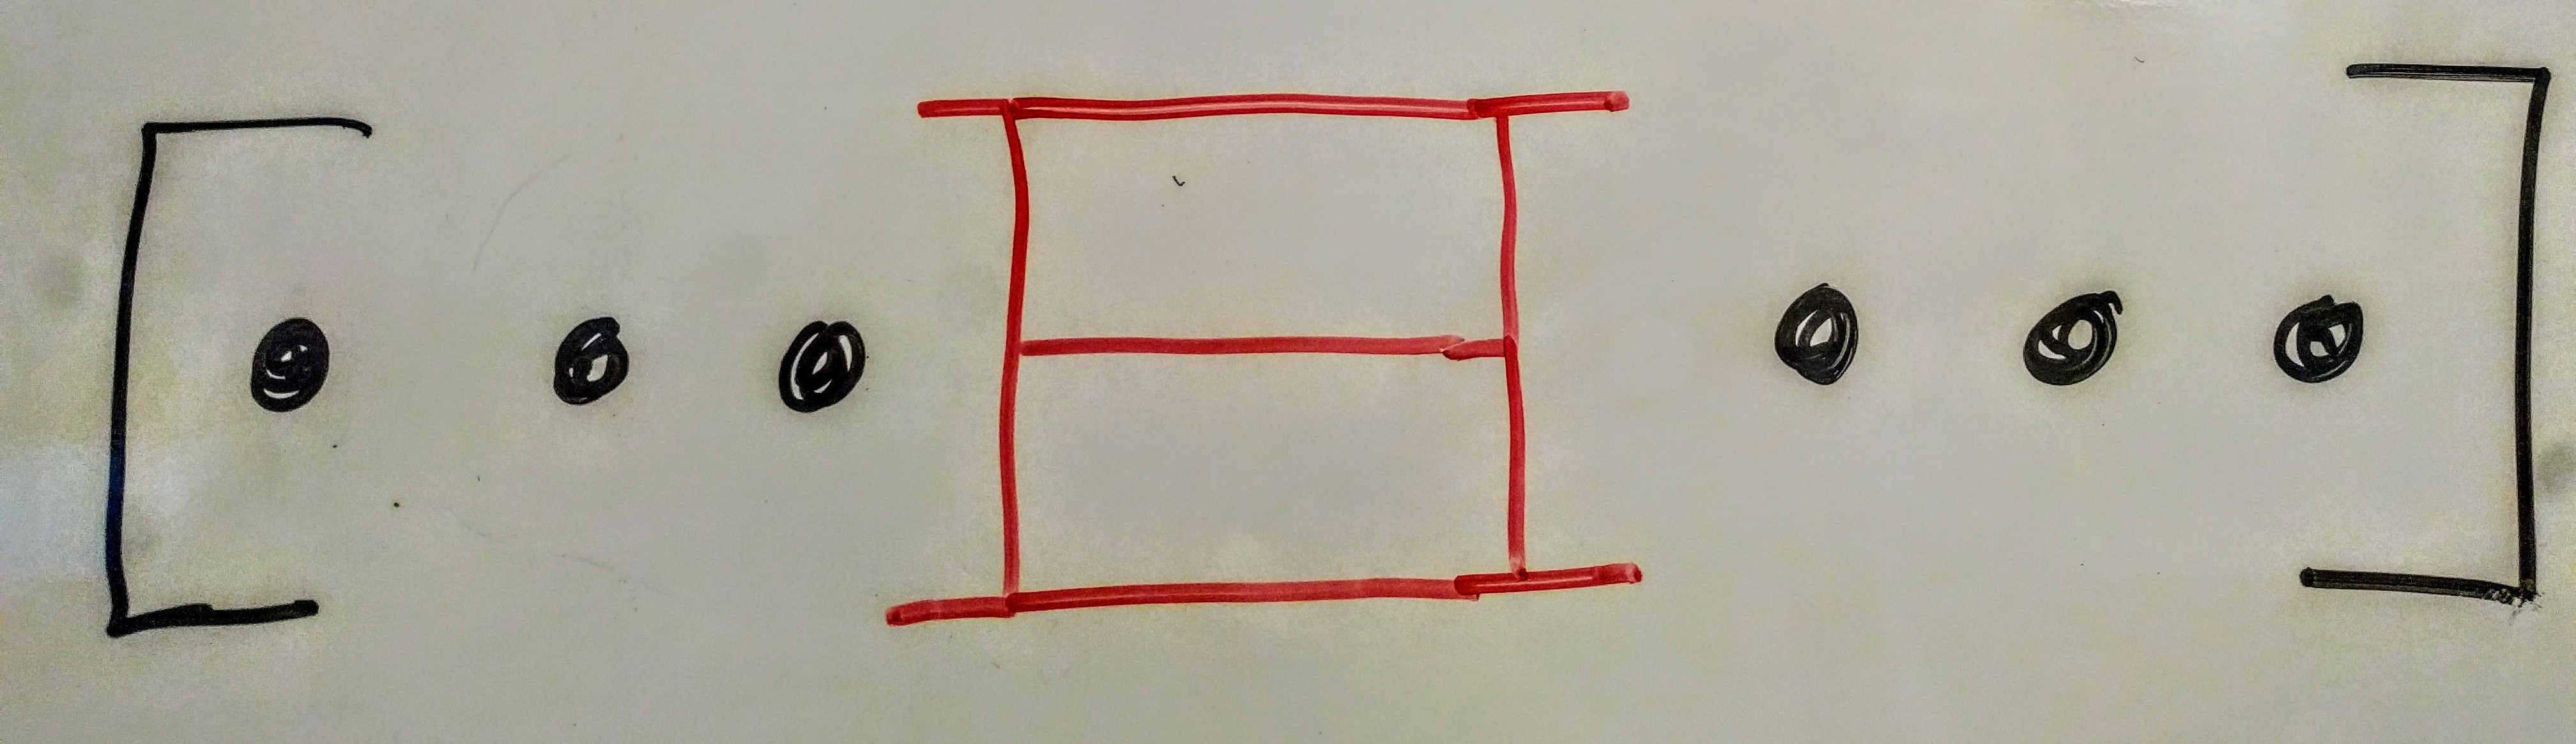
\includegraphics[width=0.5\linewidth]{images/tile2-1.jpg}
        \label{fig:b21}
    }
    \subfloat[][]{
        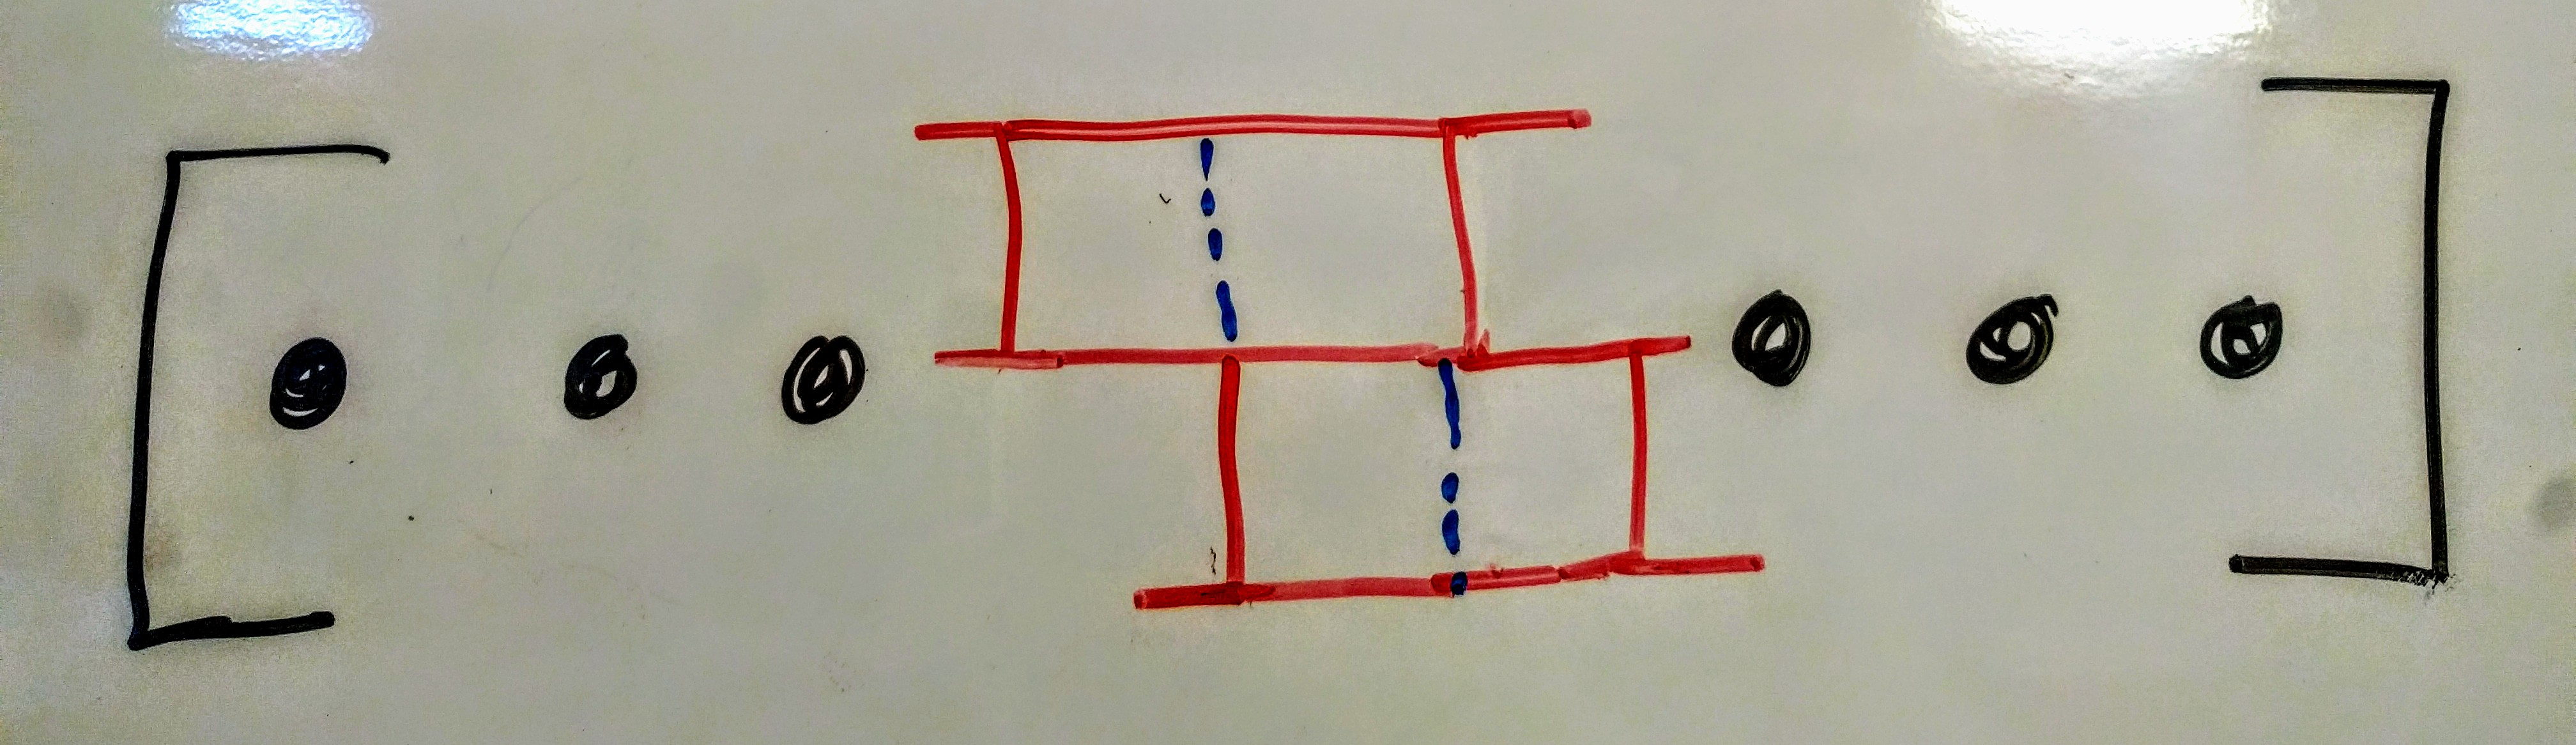
\includegraphics[width=0.5\linewidth]{images/tile2-2.jpg}
        \label{fig:b22}
    }
    \caption{Caption for this figure with two images}
    \label{fig:boundary2}
\end{figure}

Now, consider a query to the location $i$, such that all positions between $i-a$ and $i+b$ have not been queriesd so far.
So, there is a blank $2\times(a+b)$ size sub-grid that we have to sample from.
Let us consider the number of possible tilings resulting from each possible splitting boundary.
\begin{enumerate}
    \item Vertical Boundary -- This indicates that we divide the region into two sub-grids with sizes
          $2\times a$ and $2\times b$.
          So, the total number of possible tilings is exactly $F_a\cdot F_b$.
    \item Horizontal Boundary -- This indicates that we divide the region into two sub-grids with sizes
          $2\times (a-1)$ and $2\times (b-1)$.
          So, the total number of possible tilings is exactly $F_{a-1}\cdot F_{b-1}$.
\end{enumerate}

So the probabilities are computed as $\frac{F_a\cdot F_b}{F_a\cdot F_b + F_{a-1}\cdot F_{b-1}}$
and $\frac{F_{a-1}\cdot F_{b-1}}{F_a\cdot F_b + F_{a-1}\cdot F_{b-1}}$.
Now, we face the issue of approximating these fractions.
If either of the values $a$ or $b$ are less than $\Theta(\sqrt n)$,
then we can compute the exact value of the corresponding $F_a$ or $F_b$.
Otherwise, we use Lemma~\ref{lem:rat_conv} to approximate $F_a=\phi\cdot F_{a-1}$ and $F_b=\phi\cdot F_{b-1}$.
So, the probability of the vertical boundary becomes
$$
\frac{F_a\cdot F_b}{F_a\cdot F_b + F_{a-1}\cdot F_{b-1}} = \frac{\phi^2}{\phi^2+1}
$$
Similarly, the probability of a horizontal split with a top and bottom domino becomes $1/(\phi^2+1)$.
Note that this also determines the two adjacent boundaries.

The only information we needed to make this query was the extent of the un-queried interval $[i-a, i+b]$.
We can use any standard data-structure that allows insertion in positions $\{1, 2\cdots,n+1\}$,
and provides successor and predecessor queries.

Here's we can be fancy and use Van-Emde-Boas trees to get a $\Bo(\log\log n)$ query time.
However, in some cases, the exact value of a Fibonacci number still needs to be computed, and this takes $\Bo(\log n)$ time.
The faster queries only work when the new query is "far enough" ($\Bo(\log n)$ distance) away from all previous queries.



%\subsection{Permutations}

\anak{Did we try to support more information that just computing $\pi(i)$?}
[Specification]

In addition to a table (dictionary) containing all assigned values $\pi(i)$, we maintain the following binary trees,
whose nodes are generated on-the-fly in response to queries.

$T_1$: Each node of $T_1$ corresponds to a specific range of indices,
where the root represents the entire range $\{1, \ldots, N\}$,
and its two children represents each (approximately) half of the parent's range.
Each node counts the indices $i$ in the range, such that $\pi(i) = \bot$.
Initially $T_1$ only contains the root node, and the number of unassigned indices are $N$.
The children are only generated when we need to traverse down from the root; as these nodes are generated,
all of the indices in their ranges are unassigned.
Once an index becomes assigned, we simply update the information along the path in $\Bo(\log n)$ time.

$T_2$: $T_2$ is similar to $T_1$ but instead of maintaining the number of indices in the range that are still unassigned,
it maintains the number of values in the range that are still unused (have not been assigned to an index).
Similarly, we may sample an unused value or mark it as used within $\Bo(\log n)$ time.

To compute $\pi(i)$, first we check the table for $\pi(i)$ and return its value if $\pi(i)\neq\bot$.
Otherwise, sample an unused value $j$ from $T_2$ and mark that value as used.
Add $\pi(i) = j$ to the table, and mark index $i$ as used on $T_1$.

If we wish to support $\pi^{-1}(i)$, then also store the table of $\pi^{-1}(i)$.
To assign $\pi^{-1}(i)$, sample an unassigned index $j$ from $T_1$ then mark it as assigned,
add $\pi(j)=i$ and $\pi^{-1}(i)=j$ to the table, and mark the value $i$ as used on $T_2$.

\subsection{Generating Permutations with given Cyclic Structure}
We will use the technique from \cite{cyclic} to locally generate a random permutation with a given cyclic structure.
This algorithm uses two permutations $\pi$ and $\sigma$,
where $\pi$ is a uniformly random permutation and $\sigma$ is a fixed permutation with the given structure.
The resulting random permutation is formed by the composition $\pi^{-1}(\sigma(\pi(\cdot)))$.
We will generate the permutation $\pi$ as described in the previous section.;



We receive as input a list of cycle sizes \{$c_1, c_2,\cdots, c_k\}$ with the restriction that $\sum c_i = n$.
Now we need to locally generate the permutation $\sigma$ with the prescribed structure.
Define the indices $C_j = \SL{i=1}{j}c_i$ with $C_0 = 0$.
We will construct the cycle corresponding to $c_i$ as all the elements in the interval $\{c_{i-1}+1,c_{i-1}+2,\cdots,c_i\}$.

Of course we will not be computing $\sigma$ explicitly.
Instead, we will pre-compute the $C_j$ indices, and when given a query $\sigma(x)$,
we binary search amongst $C_j$ to find the cycle that $x$ belongs to.
Then we can report the value of $\sigma(x)$ accordingly.

So, we can now compose the generator oracles for $\pi$, $\sigma$, and $\pi^{-1}$ to get the full generator. 


\section{Catalan Objects}%
\label{sec:catalan_objects}


\subsection{Dyck Paths}
\label{sub:dyck_paths}


Dyck paths are one interpretation of the Catalan numbers.
Here, we will instead consider a more general form of Dyck Paths, which correspond to numbers in the \textit{Catalan Trapezoid}.

A Dyck path can be constructed as a $1D$ random walk with $2n$ steps,
where the ends of the walk are pinned to zero (Figure~\ref{fig:dyck}).
This path also has the additional restriction that the walk can never reach negative values.
The number of possible Dyck paths is the $n^{th}$ Catalan number --
$$C_n = \frac{1}{n+1}\cdot {2n\choose n}$$
We will attempt to support queries to a uniformly random instance of a Dyck path.
Specifically, we will want to query the position of the $i^{th}$ index.

\subsection{Catalan Trapezoid}
First, we define Catalan trapezoids as presented in \cite{trap}.
Let $C_k(n,m)$ be the $(n,m)^{th}$ entry of the Catalan trapezoid of order $k$, where $C_1(n,m)$ corresponds to the Catalan triangle.

The interpretation is as follows. Consider a sequence of $n$ $(+1)$s and $m$ $(-1)$,
such that the sum of any initial sub-string is not less than $1-k$.
This means that we start our Dyck path at a height of $k-1$, and we are never allowed to cross below zero.
The total number of such paths is exactly $C_k(n,m)$.

Now, we state a result from \cite{trap} without proof
$$
C_k(n,m)=
\begin{cases}
{n+m}\choose m &0\le m<k\\
{{n+m}\choose{m}} - {{n+m}\choose{m-k}} &k\le m<n+k-1\\
0 &m>n+k-1
\end{cases}
$$

\subsection{Generating Dyck Paths}
Our general recursive step is as follows.
We consider a sequence of length $2S$ comprising of $2U$ up moves ($+1$) and $2D$ down moves ($-1$).
Additionally, the sum of any initial sequence {\color{red} prefix?} canon be less than $k-1$.
Without loss of generality, let's assume that $2D\le S$. If this were not the case,
we could simply flip the sequence and negate the elements.
This essentially means that the overall Dyck path is non-decreasing.

\begin{lemma}
$S-2D = \Bo(\log n\sqrt S) \implies U-D = \Bo(\log n\sqrt S)$
\label{lem:dyck_var0}
\end{lemma}

We want to sample the height of this path after $S$ steps.
This is the same as sampling the number of $(+1)$s that get assigned to the first half of the elements in the sequence.
We define $p_d$ as the probability that exactly $D-d$ $(-1)$s get assigned to the first half.
This means that exactly $U+d$ $(+1)$s get assigned to the first half.
Consequently, the second half will contain exactly $D+d$ $(-1)$s and $U-d$ $(+1)$s.

Let us first compute this probability.
$$
p_d = \frac{D_{left}\cdot D_{right}}{D_{tot}}
$$
Where $D_{left}$ denotes the number of valid starting sequences (first half)
and $D_{right}$ denotes the number of valid ending sequences.
Here, \textit{valid} means that each half sequence gets the appropriate number of ups and downs
and the initial sums never drop below $1-k$.
For, $D_{right}$, we will start the Dyck path from the end of the $2S$ sequence.
In this case the invalidation threshold will be a different $k'$.
This $k'$ is the final height of the $2S$ sequence. So, $k'=k+2U-2D = k+4S-2D$. We will use this fact extensively moving forward.

Also, $D_{tot}$ is the total number of possible sequences of length $2S$ , given the initial conditions.
This value is considered by constructing paths in the original direction i.e. the value of $k$ is the same.

\subsection{The Simple Case}
The problem of sampling reduces to the binomial sampling case when $k > \mathcal{O}(\log n)\sqrt S$ for some constant $c$.
In this case, the we can simply approximate the probability as
$$
\frac{{{S}\choose{D-d}}\cdot{{S}\choose{D+d}}}{{{2S}\choose{2D}}}
$$
This is because the random paths will not have initial sums less than $1-k$ with high probability.
Note that this uses the assumption that we have an increasing path.

\subsection{Path Segments Close to Zero}
The problem arises when we $k <\mathcal{O}(\log n)\sqrt{S}$. In this case we need to compute the actual probability,
Using the formula from \cite{trap}, we find that.
\begin{align}
D_{left} = {{S}\choose{D-d}}-{{S}\choose{D-d-k}} &&D_{right} = {{S}\choose{U-d}}-{{S}\choose{U-d-k'}}
\end{align}
Here, $k' = k+2U-2D$, and so $k' = \Bo(\log n)\sqrt S$.\todo{prove using Lemma~\ref{lem:dyck_var0}}

Finally, we compute the total number of Dyck paths as
$$
D_{tot} = {{2S}\choose{2D}}-{{2S}\choose{2D-k}}
$$

Now, we are going to use the following Lemma from \cite{huge}.
\begin{lemma}
\label{lem:huge}
Let $\{p_i\}$ and $\{q_i\}$ be distributions satisfying the following conditions
\begin{enumerate}
    \item There is a poly-time algorithm to approximate $p_i$ and $q_i$ up to $\pm n^{-2}$
    \item Generating an index $i$ according to $q_i$ is closely implementable.
    \item There exists a $poly(log n)$-time recognizable set $S$ such that
    \begin{itemize}
        \item $1-\SL{i\in S}{} p_i$ is negligible
        \item There exists a constant $c$ such that for every $i$, it holds that $p_i\le \log^{\mathcal{O}(1)} n\cdot q_i$
    \end{itemize}
\end{enumerate}
Then, generating an index $i$ according to the distribution $\{p_i\}$ is closely-implementable.
\end{lemma}

In this process, we will first disregard all values of $d$ where $|d|>\Theta(\sqrt S)$.
The probability mass associated with these values can be shown to be negligible \todo{bound variance of path}.

Next, we will construct an appropriate $\{q_i\}$ and show that $p_d < \log^{\mathcal{O}(1)} n\cdot q_d$
for all $|d|<\Theta(\sqrt S)$ and some constant $c$.
We will use the following distribution
$$
q_d = \frac{{S\choose D-d}\cdot{S\choose D+d}}{{2S\choose 2D}} = \frac{{S\choose D-d}\cdot{S\choose U-d}}{{2S\choose 2D}}
$$
It is shown in \cite{huge} that this distribution is closely implementable.

\begin{lemma}
First we show that $D_{left} \le \frac{c_1\cdot k}{\sqrt{S}}\cdot{{S}\choose{D-d}}$ for some constant $c_1$.
\end{lemma}
\begin{proof}
This involves some simple manipulations.
\begin{align}
D_{left} &= {{S}\choose{D-d}}-{{S}\choose{D-d-k}}\\
&= {{S}\choose{D-d}}\cdot \left[1-\frac{(D-d)(D-d-1)\cdots(D-d-k+1)}{(S-D-d+k)(S-D-d+k-1)\cdots(S-D-d+1)}\right]\\
&\le {{S}\choose{D-d}}\cdot \left[1-\left(\frac{D-d-k+1}{S-D+d+k}\right)^k\right]\\
&\le {{S}\choose{D-d}}\cdot \left[1-\left(\frac{U+d+k-(U-D+d+k-1)}{U+d+k}\right)^k\right]\\
&\le {{S}\choose{D-d}}\cdot \left[1-\left(\frac{U+d+k-\Bo(\sqrt{U})}{U+d+k}\right)^k\right]\\
&\le \frac{k}{\Theta(\sqrt{S})}\cdot{{S}\choose{D-d}}
\end{align}
\end{proof}

\begin{lemma}
Similarly, we show that $D_{right} < \frac{c_2\cdot k'}{\sqrt{S}}\cdot{{S}\choose{U-d}}$ for some constant $c_2$.
\end{lemma}
\begin{proof}
\begin{align}
D_{right} &= {{S}\choose{U-d}}-{{S}\choose{U-d-k'}}\\
&= {{S}\choose{U-d}}\cdot \left[1-\frac{(U-d)(U-d-1)\cdots(U-d-k'+1)}{(S-U-d+k')(S-U-d+k'-1)\cdots(S-U-d+1)}\right]\\
&\le {{S}\choose{U-d}}\cdot \left[1-\left(\frac{U-d-k'+1}{S-U+d+k'}\right)^{k'}\right]\\
&\le {{S}\choose{U-d}}\cdot \left[1-\left(\frac{2D-U-d-k+1}{2U-D+k+d}\right)^{k'}\right]\\
&\le {{S}\choose{U-d}}\cdot \left[1-\left(\frac{U+k+d - (2U-2D+2d+2k-1)}{U+k+d}\right)^{k'}\right]\\
&\le {{S}\choose{U-d}}\cdot \left[1-\left(\frac{U+k+d - \Bo(\sqrt U)}{U+k+d}\right)^{k'}\right]\\
&\le \frac{k'}{\Theta(\sqrt{S})}\cdot{{S}\choose{U-d}}
\end{align}
\end{proof}

Finally, we need to lower bound the value of $D_{tot}$.

\begin{lemma}
We claim that $D_{tot} < \frac{c_3\cdot k\cdot k'}{S}\cdot{{2S}\choose{2D}}$ for some constant $c_3$.
\end{lemma}
\begin{proof}
\begin{align}
D_{tot} &= {{2S}\choose{2D}}-{{2S}\choose{2D-k}}\\
&= {{2S}\choose{2D}}\cdot \left[1-\frac{(2D)(2D-1)\cdots(2D-k+1)}{(2S-2D+k)(2S-2D+k-1)\cdots(2S-2D+1)}\right]\\
&\ge {{2S}\choose{2D}}\cdot \left[1-\left(\frac{2D-k+1}{2S-2D+1}\right)^k\right]\\
&\ge {{2S}\choose{2D}}\cdot \left[1-\left(\frac{2U-(2U-2D+k-1)}{2U+1}\right)^k\right]\\
&\ge {{2S}\choose{2D}}\cdot \left[1-\left(\frac{(2U+1)-k'}{2U+1}\right)^k\right]\\
&\ge \frac{k\cdot k'}{\Theta(S)}\cdot{{2S}\choose{2D}}
\end{align}
\end{proof}

\begin{theorem}
We can now put these lemmas together to show that $p_d/q_d \le c = c_1\cdot c_2/c_3 = \Theta(1)$.
This satisfies all the conditions of Lemma~\ref{lem:huge} from \cite{huge}.
We simply need to set the accept probability less than $p_d/(c\cdot q_d)$.
\end{theorem}



\bibliographystyle{alpha}

\bibliography{bib}


\end{document}
